\documentclass[compress]{beamer}
\usepackage[danish]{babel}
\usepackage[latin1]{inputenc}
\usepackage{listings}

% \usepackage{beamerthemesplit}
%\usepackage{graphicx}
\usetheme{Darmstadt}
%\usetheme{PaloAlto}
%\usetheme{Berkeley}
%\usetheme{Frankfurt}
%\usetheme{Hannover}

%\usepackage{beamerarticle}

\setbeamerfont{block body}{size=\scriptsize}

\usepackage{SHmathnot}
\usepackage{natbib}
%\usepackage{color,amsmath,amsfonts}
\usepackage{ISMLS}

\setbeamertemplate{footline}[page number]



%\makeatletter
%\AtBeginPart{\beamer@tocsectionnumber=0\relax\c@section=0}
%\makeatother

\title{\texttt{Rmarkup} -- a very simple tool for literate programming
}

\author{S�ren H�jsgaard}
\institute{Department of Mathematical Sciences \\ Aalborg University
  \\ Denmark \\ \ \\ useR! 2012 conference \\ Nashville, TN, USA}
\newenvironment{sframe}
                {\begin{frame} [containsverbatim] }
                {\hfill  \end{frame}}

\newenvironment{sblock}
                 {\begin{block} {R-code} }
                 {\hfill  \end{block}}

              
\usepackage{Sweave}
\begin{document}

\frame{\titlepage}

\parskip4pt
\section{Contents}
\begin{frame}
 \setcounter{framenumber}{1}
  \tableofcontents  
\end{frame}




\lstset{language=R,
  basicstyle=\tiny, 
%  numbers=left,
  frame=single,
  basicstyle=\ttfamily,
  keywordstyle=\color{blue},
  commentstyle=\color{darkblue}
  %backgroundcolor=\color{lightpurple}
}


\def\proglang#1{{#1}}
\def\pkg#1{{\bf #1}}
\def\doby{\pkg{doBy}}
\def\odfweave{\pkg{odfWeave}}

\def\code#1{\texttt{#1}}
\def\shd#1{\footnote{SHD: #1}}
\def\rep{\code{Rmarkup()}}
\def\R{\proglang{R}}

\def\rmark{\texttt{Rmarkup()}}
\def\sweave{\code{Sweave()}}


\section{What is \rmark?}
\label{sec:what-rmark}

\begin{sframe}
%\frametitle{What is \rmark}
  
  \begin{itemize}

  \item \rmark\ very leight weight tool for literate programming.

  \item Not unlike \code{R Markdown} presented earlier by JJ Allarie.
    
  \item Input: Plain text file containing
    \begin{itemize}
    \item  \proglang{R} code

    \item Comment lines (starting with \#\#) with descriptive text. 
      Simple text markups are implemented.
    \end{itemize}
    
    
  \item Output: HTML document containing 
    \begin{itemize}
    \item  Descriptive text (with possible markups),
    \item program code together with
    \item graphics and results from the computations.
    \end{itemize}
    

  \item Genesis: Teaching \R\ in life sciences
  \item The \rmark\ function is in the \pkg{doBy} package.
    
  \item \rmark\ is implemented by using the
    \code{RweaveHTML} driver in the \pkg{R2HTML}%, \citep{R2HTML}.

\end{itemize}

\end{sframe}

\subsection{Example}
\label{sec:example}
\begin{sframe}
  
  {\scriptsize \lstinputlisting{SweaveEx1.R}} 

\end{sframe}

\begin{sframe}

  \begin{itemize}
  \item Run \rmark\ as:


\begin{Schunk}
\begin{Sinput}
R> Rmarkup("SweaveEx1.R", 
+      encoding = "latin1",     # because of the '�'s
+      cssfile  = "R2HTML.css") # optional css file
\end{Sinput}
\end{Schunk}


\item Will produce \code{SweaveEx1.html} in working directory (where
the \code{css} file must reside).
  
\item If a pdf-file is needed, the utility \code{wkhtmltopdf} is useful, see
\begin{quote}
\url{http://code.google.com/p/wkhtmltopdf/}  
\end{quote}


\item Simply do:

\begin{Schunk}
\begin{Soutput}
wkhtmltopdf SweaveEx1.html SweaveEx1.pdf
\end{Soutput}
\end{Schunk}

  \end{itemize}

\end{sframe}

{
\usebackgroundtemplate{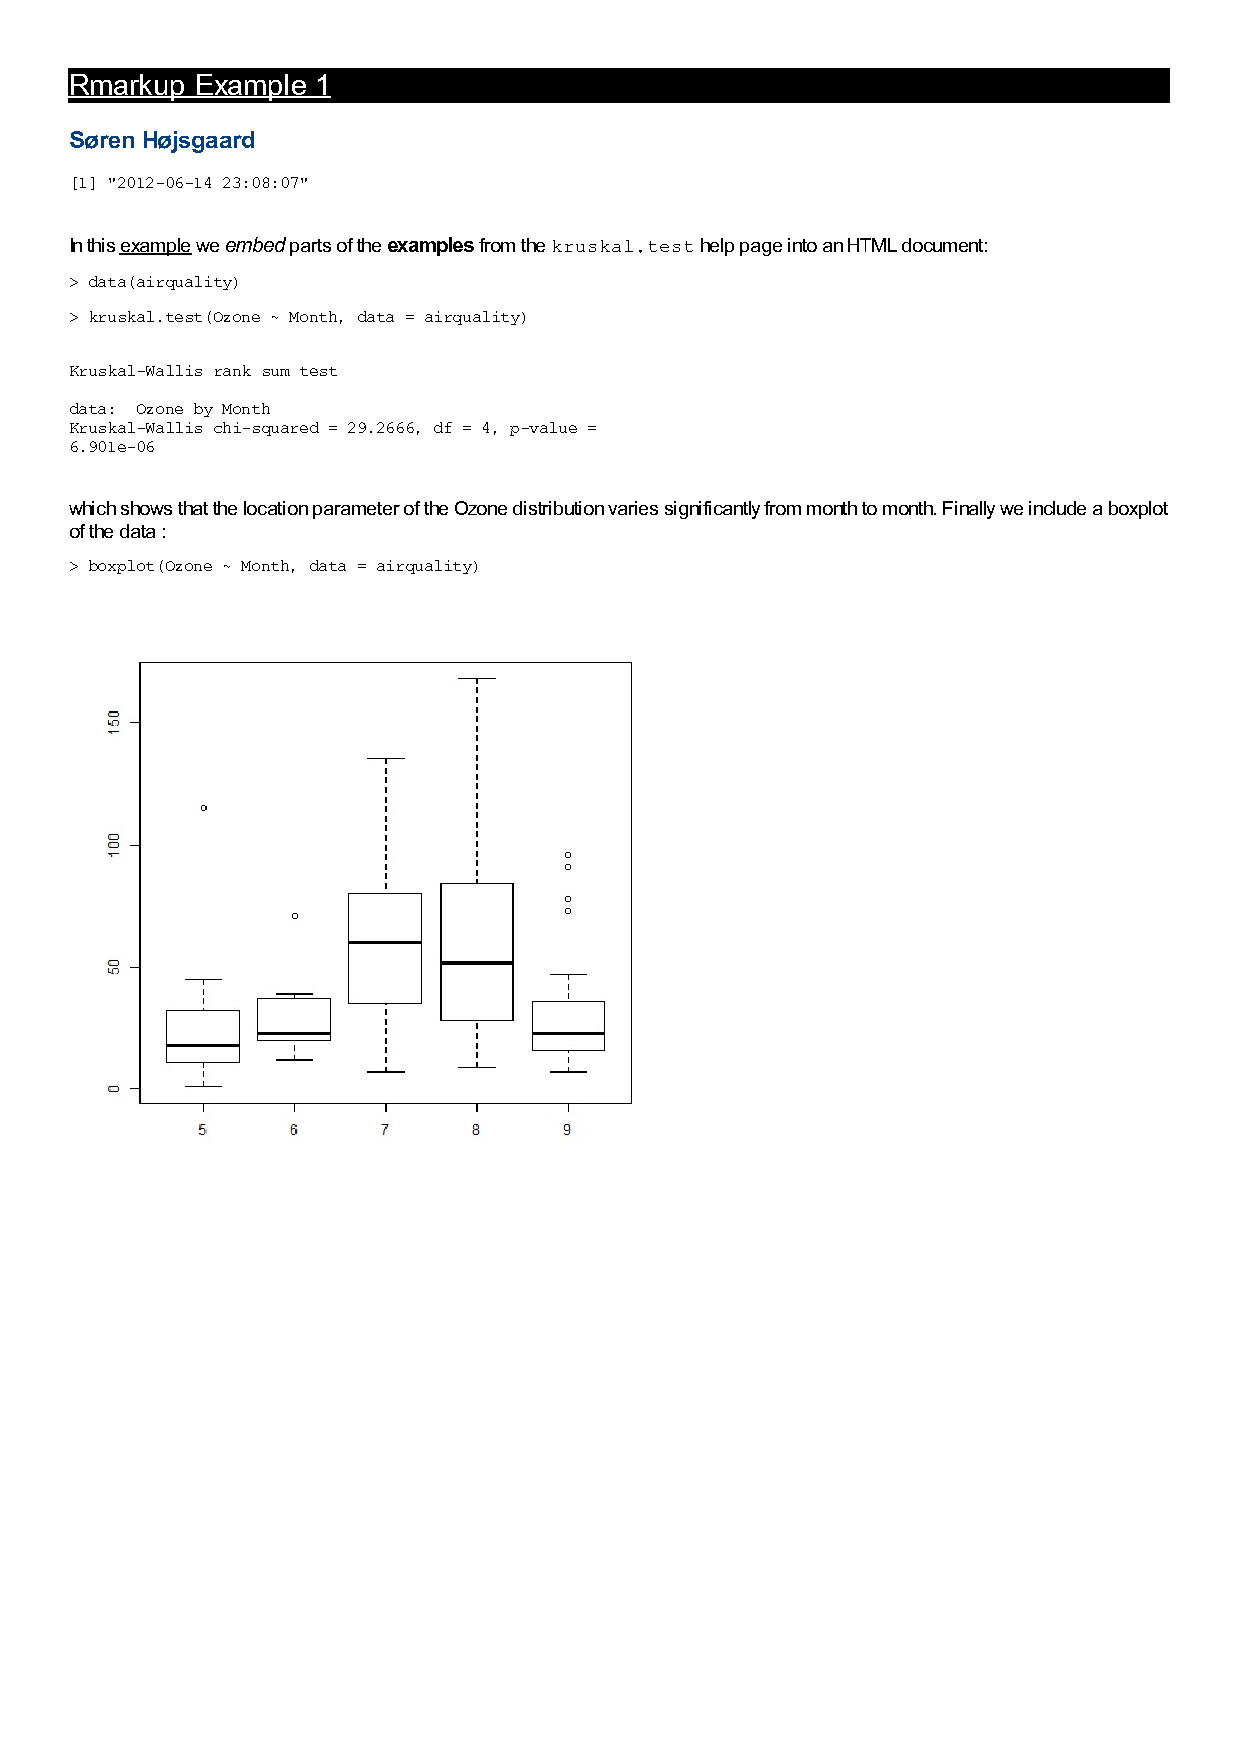
\includegraphics[width=0.9\paperwidth]{SweaveEx1}}
\begin{frame}[plain]
\end{frame}
}




\section{Markup of R-script}
\label{sec:markup}

\begin{sframe}
All text lines start with one or more hashes (\code{\#}) because these
lines are to be regarded as comments by \R.

Lines starting with: 

\begin{itemize}
\item One or two hashes: Regarded as a text which
  is transferred (possibly after some additional processing; see below)
  to the resulting HTML document.
\item Three or more hashes: Not transferred to the HTML
  document. (This is useful e.g. for TODOs).
\end{itemize}
  
\end{sframe}



\subsection{Headings and text beautifiers}
\begin{sframe}
  \begin{itemize}
  \item     \rmark\ allows some markup facilities for the text
    inspired by \code{txt2tags} markups (see \url{http://txt2tags.org/}).
  \item Headings at different font
    sizes are produced with (there can be 6 levels of headings):

    \verb'= Title level 1 =', \verb'== Title level 2 ==', ...

  \item The time of creation of the HTML document is produced with
  
    \verb'%%date'.

  \end{itemize}
\end{sframe}


\begin{sframe}
  
\begin{itemize}

\item{Beautifiers:
    
    {\bf boldface},
    {\it italics},
    \underline{underline},
    \code{monospace}
    :}
  

\item Produced with:

  \verb'**'boldface\verb'**',  \verb'//'italics\verb'//'
  \verb'__'underline\verb'__', \verb'&&'monospace\verb'&&'

\item Beautifiers can be combined in any way, e.g.

  \verb'**__'some text\verb'__**'.

\item Beautifiers can be used in the headings.

\end{itemize}
\end{sframe}




\subsection{Using noweb markups}
\label{sec:using-noweb-markups}

\begin{sframe}

  \begin{itemize}
  \item 
Writing 
\begin{verbatim}
## @@
data(airquality)
## @
\end{verbatim}

is equivalent to 

\begin{verbatim}
## <<>>=
data(airquality)
## @
\end{verbatim}


\item Other valid specs can go into \verb'<<>>'.

\end{itemize}
  
  
  
\end{sframe}

\begin{sframe}
  \begin{itemize}
  \item Writing
\begin{verbatim}
## @@@
plot(airquality)
## @
\end{verbatim}

is equivalent to 

\begin{verbatim}
## <<fig=T>>=
data(airquality)
## @
\end{verbatim}
  

\item Other valid specs can go into \verb'<<>>'.
\end{itemize}
  
\end{sframe}

\subsection{Controlling graphics and using Sexpr\{\}}
\label{sec:controlling-graphics}

\begin{sframe}
  
  {\scriptsize \lstinputlisting{script/SweaveEx2.R}} 

\end{sframe}


\begin{sframe}

Run \rmark\ as:
\begin{Schunk}
\begin{Sinput}
R> Rmarkup("script/SweaveEx2.R", 
+          destdir  = "./report", 
+          encoding = "latin1",
+          cssfile  = "R2HTML.css",
+          parms = list(height = 200, width = 200)
+          )
\end{Sinput}
\end{Schunk}
  
  


\end{sframe}

% \begin{sframe}
%   \begin{figure}
%     \centering
%     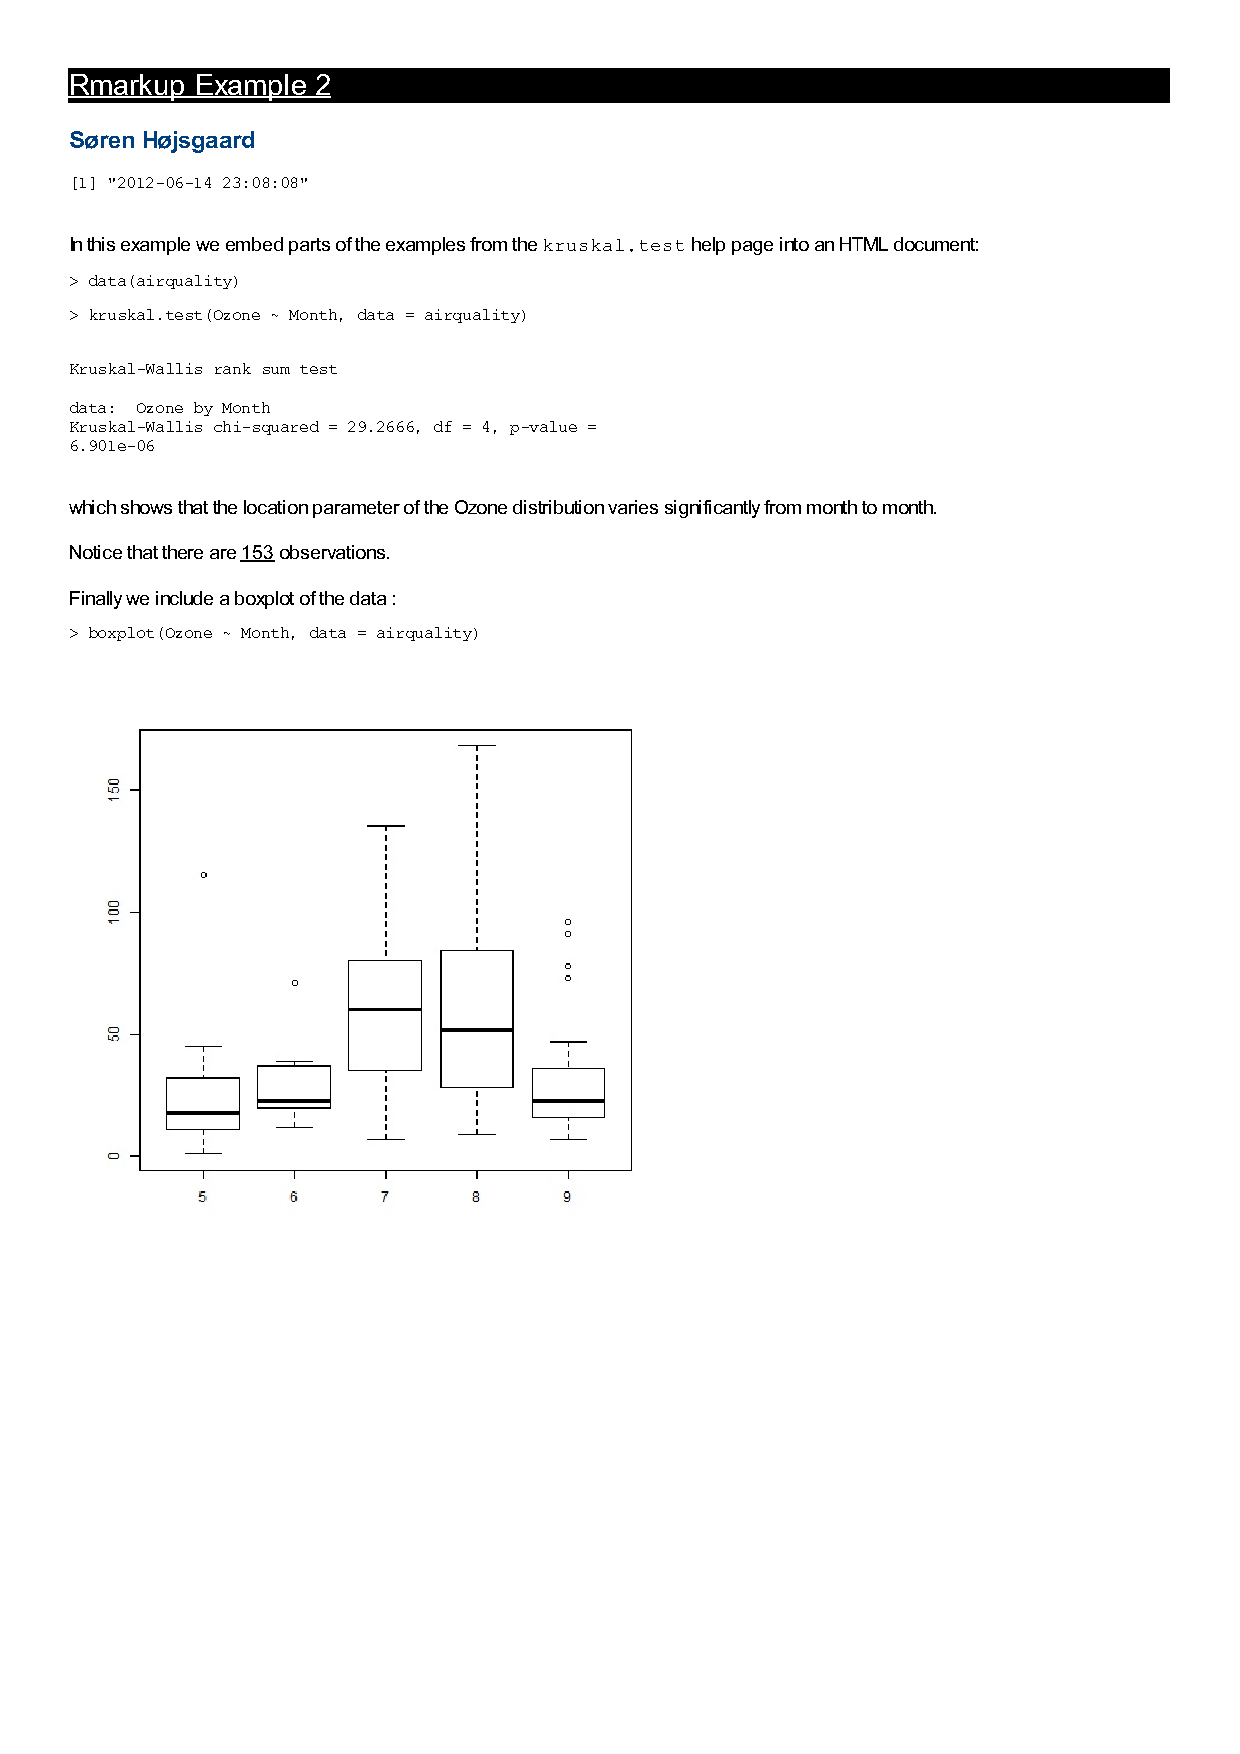
\includegraphics{report/SweaveEx2}
%     \caption{ss}
%     \label{fig:ff}
%   \end{figure}
% \end{sframe}


{
\usebackgroundtemplate{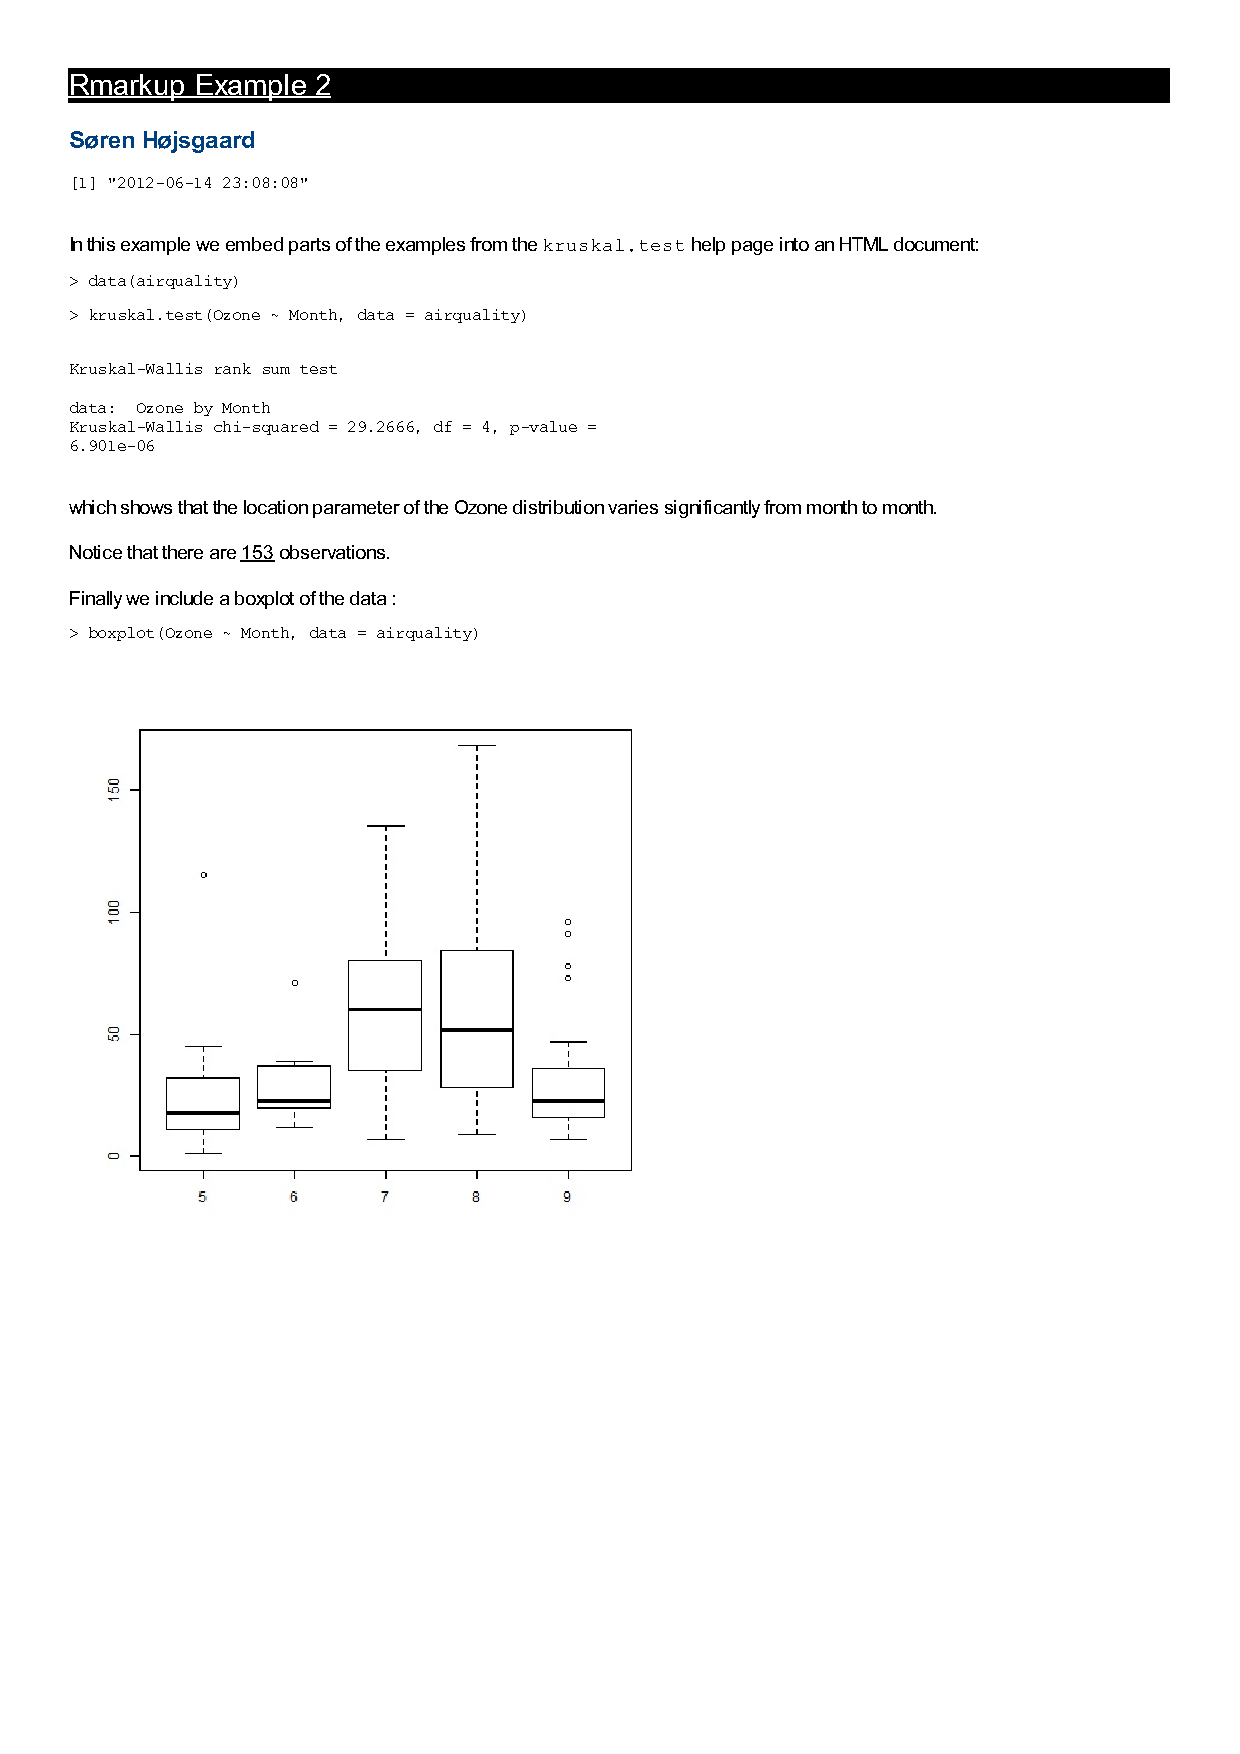
\includegraphics[width=0.9\paperwidth]{report/SweaveEx2}}
\begin{frame}[plain]
\end{frame}
}


\subsection{Restrictions}
\label{sec:restrictions}

\begin{sframe}
\begin{itemize}
\item A text markup must be completed in one line 
  
\item Example: a heading in a large font can be obtained with
\begin{verbatim}
## = HERE COMES A TITLE =
\end{verbatim}

\item -- whereas this is not obtained if one writes e.g.
\begin{verbatim}
## =
##   HERE COMES A TITLE
## =
\end{verbatim}

\item Comments in code chunks will not appear in output
\end{itemize}
\end{sframe}


\section{Winding up}
\label{sec:winding-up}


\subsection{Genesis of \rmark}
\label{sec:why-rmarkup}
        
\begin{sframe}

  
\rmark\ grew out of teaching \proglang{R} to graduate students
    and others in the life sciences.

  \begin{itemize}
  \item Mainly Microsoft Office users 
    
  \item Learning \R\ itself is a hurdle. 

  \item Hesitant to install to much software on their computers. 
    Installing \proglang{R} and a suitable editor (e.g.\ \proglang{Notepad++} 
    for Windows users) is about as
    much as we can ask for.
  \item (\code{Rstudio} could well be a better choice today.)

  \item Over the top to ask students to learn \LaTeX\ (also irrelevant;
    they collaborate on / submit papers in MS Office format)

  \item Even \odfweave\ is problematic, as there is no Windows binary
    on CRAN (depends on \pkg{XML}?).
    
  \end{itemize}
  
\end{sframe}



\subsection{Added bonus?}
\label{sec:added-bonus}

\begin{sframe}

  
  Why would anyone possibly want to use \rmark\ when so many fancy
  literate programming tools are available?
    
  \begin{itemize}

  \item Often we work with a script file as a sandbox for
    e.g. data manipulation tasks, exploratory data analysis etc.
  \item To document the work one may choose to create a \LaTeX file with 
    describing such activities using
    \code{Sweave}.
  \item But most people maintain their \R\ scripts. So one may have 
    two different files describing essentially the same tasks.
  \item \rmark\ allows one to create a reasonably nice looking report
    from an \R\ script itself.
  \item Hence the task of
    documenting the work (in particular the more tedious parts of the
    work) is more likely to be done.

  \end{itemize}
  
\end{sframe}

\subsection{Future of \rmark\ and final remarks}
\label{sec:future-rmark}

\begin{sframe}
  
  \begin{itemize}

  \item \rmark\ may be useful in teaching students  ``good habbits''
    
  \item \rmark\ may help others doing the same...

  \item \rmark\ will never be developed to a fancy tools with all
    sorts of bells and whistles.
  

  \item Still, open to suggestions - to pick the ``low hanging fruits''

  \item A small demo!!
  \end{itemize}

  \begin{center}
    
    {\Large Thank you for your attention!}
  \end{center}
  
\end{sframe}

% @ 
% <<eval=F>>=
% unlink("report/*.pdf")
% @ %def 





\end{document}

